\chapter{The categorical origins of entropy}
\lbl{ch:cat}
\index{category theory}


In this chapter, we describe a general category-theoretic construction
which, when given as input the real line and the notion of finite
probability distribution, automatically produces as output the notion of
Shannon entropy (Figure~\ref{fig:machines}).

\begin{figure}
\centering
\lengths
\begin{picture}(54,60)
\cell{27}{30}{c}{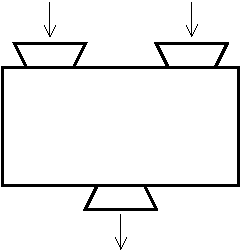
\includegraphics[height=40\unitlength]{machinem}}
\cell{27}{35}{c}{internal algebras}
\cell{27}{30}{c}{in a categorical algebra}
\cell{27}{25}{c}{for an operad}
\cell{16}{52}{c}{$(\Delta_n)$}
\cell{38}{52}{c}{$\R$}
\cell{27}{7}{c}{Shannon entropy}
\cell{27}{-1}{b}{(a)}
\end{picture}%
\hspace*{12mm}%
\begin{picture}(54,60)
\cell{27}{30}{c}{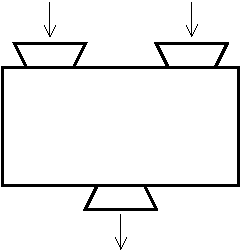
\includegraphics[height=40\unitlength]{machinem}}
\cell{27}{35}{c}{internal algebras}
\cell{27}{30}{c}{in a categorical algebra}
\cell{27}{25}{c}{for an operad}
\cell{16}{52}{c}{$(1)$}
\cell{38}{52}{c}{$\cat{V}$}
\cell{27}{7}{c}{monoid in $\cat{V}$\vphantom{y}}
\cell{27}{-1}{b}{(b)}
\end{picture}%
\caption{Schematic illustration of the main result of this chapter,
  Theorem~\ref{thm:cat-ent}.  There is a general categorical machine
  which \hardref{(a)}~when given as input the simplices $(\Delta_n)$ and
  the real line, produces as output the notion of Shannon entropy, and
  \hardref{(b)}~when given as input the one-point set $1$ and a monoidal
  category $\cat{V}$, produces as output the notion of monoid in $\cat{V}$.}
\lbl{fig:machines}
\index{internal algebra!schematic illustration}
\end{figure}

The moral of this result is that even in the pure-mathematical heartlands
of algebra and topology, entropy is inescapable.%
%
\index{entropy!inescapable@is inescapable}
% 
This may come as a surprise: for although entropy is a major concept in
many branches of science, an algebraist, topologist or category
theorist can easily go a lifetime without encountering entropy of any
kind.

Yet the categorical construction described here is entirely general and
natural.  It is not tailor-made for this particular purpose.  Other
familiar inputs produce familiar outputs.  And the inputs that we give to
the construction here, the real line $\R$ and the standard topological
simplices $\Delta_n$, are fundamental objects of pure mathematics.  So, we
are all but forced to accept Shannon entropy as a natural concept in
pure mathematics too~-- quite independently of any motivation in terms of
information, diversity, thermodynamics, and so on.

The categorical construction involves operads and their algebras.  The
first two sections set out some standard definitions, beginning
with operads and algebras themselves in Section~\ref{sec:opds}.  For an
operad $P$, there are notions of categorical $P$-algebra $\scat{A}$ (a
category acted on by $P$) and of internal algebra in $\scat{A}$.  With
these definitions in place (Section~\ref{sec:cat-int-alg}), we can fulfil
the promise of the first paragraph above (Theorem~\ref{thm:cat-ent}).
Specifically, we show that for the operad $\Delta$ of simplices and the
categorical $\Delta$-algebra $\R$, the internal algebras in $\R$ are
precisely the scalar multiples of Shannon entropy.

In the final section, we describe the free categorical $\Delta$-algebra
containing an internal algebra.  The result proved is analogous to the
classical theorem that the free monoidal category containing a monoid is
the category of finite totally ordered sets.  To reach this result involves
a further climb up the mountain of categorical abstraction.  But at the end
of the path is a characterization of information loss that is entirely
concrete. It is almost exactly the characterization theorem of
Chapter~\ref{ch:loss}.

This chapter assumes some knowledge of category theory, including the
concepts of product in a category, monoid in a monoidal category, and
internal category in a category with finite limits.  


\section{Operads and their algebras}
\lbl{sec:opds}


An operad is a system of abstract operations, somewhat like an algebraic
theory in the sense of universal algebra, but more restricted in nature.
Operads first emerged in algebraic topology (Boardman and Vogt~\cite{BoVo};
May~\cite{MayGIL}), while independently, the more general notion of
multicategory was being developed in categorical logic
(Lambek~\cite{LambDSC2}).  Nowadays, operads (like many other categorical
structures) have found application in a very wide range of subjects, from
algebra to theoretical physics.  Some samples of such applications can be
found in Kontsevich~\cite{KontOMD}, Loday and Vallette~\cite{LoVa}, and
Markl, Shnider and Stasheff~\cite{MSS}.

Many introductions to operads are available, such as \cite{LoVa},
\cite{MSS}, and Chapter~2 of~\cite{HOHC}.  Here we give only the definitions
and results that are needed in order to reach our goal.

An operad consists of a sequence $(P_n)_{n \geq 0}$ of sets equipped with
certain algebraic structure obeying certain laws.  It is
useful to view the elements $\theta$ of $P_n$ as abstract operations with
$n$ inputs and one output, as in Figure~\ref{fig:opd-opn}.
% 
\begin{figure}
\centering
\lengths
\begin{picture}(120,16)
\cell{60}{8}{c}{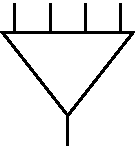
\includegraphics[height=16\unitlength]{transistor}}
\cell{60}{9}{c}{\normalsize$\theta$}
\end{picture}
\caption{An element $\theta \in P_4$ of an operad $P$.}
\lbl{fig:opd-opn}
\end{figure}
% 
A typical example will be given by $P_n = \cat{A}(A^{\otimes n}, A)$, for
any object $A$ of a monoidal category $\cat{A}$.  The algebraic structure
on the sequence of sets $(P_n)_{n \geq 0}$, and the equational laws that
this structure obeys, are exactly those suggested by this example.

\begin{figure}
\centering
\lengths
\begin{picture}(120,41.4)
\cell{35}{20.7}{c}{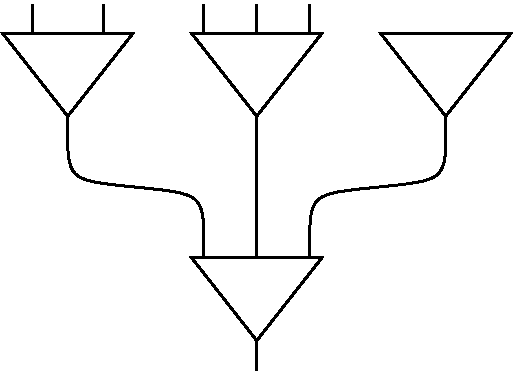
\includegraphics[height=41.4\unitlength]{transistor_tree}}
\cell{80}{20.7}{c}{\Large$\mapsto$}
\cell{105}{20.7}{c}{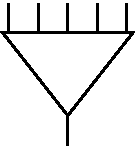
\includegraphics[height=16\unitlength]{transistor5}}
\cell{35}{9}{c}{\normalsize$\theta$}
\cell{15}{34}{c}{\normalsize$\phi^1$}
\cell{36}{34}{c}{\normalsize$\phi^2$}
\cell{56.5}{34}{c}{\normalsize$\phi^3$}
\cell{105}{10}{c}{\normalsize$\theta\of(\phi^1, \phi^2, \phi^3)$}
\end{picture}
\caption{Composition in an operad: $\theta \in P_3$ composes with $\phi^1
  \in P_2$, $\phi^2 \in P_3$ and $\phi^3 \in P_0$ to give $\theta \of
  (\phi^1, \phi^2, \phi^3) \in P_5$.}  
\lbl{fig:opd-defn}
\end{figure}

\begin{defn}
\lbl{defn:opd}
An \dmph{operad} $P$ consists of:
% 
\begin{itemize}
\item 
a sequence $(P_n)_{n \geq 0}$ of sets;

\item
for each $n, k_1, \ldots, k_n \geq 0$, a function
% 
\begin{equation}
\lbl{eq:opd-comp}
P_n \times P_{k_1} \times \cdots \times P_{k_n} 
\to
P_{k_1 + \cdots + k_n}
\end{equation}
% 
(Figure~\ref{fig:opd-defn}), called \demph{composition}%
%
\index{composition!operad@in operad}
% 
and written as
\[
(\theta, \phi^1, \ldots, \phi^n) \mapsto 
\theta \of (\phi^1, \ldots, \phi^n);
\ntn{compopd}
\]

\item
an element $1_P\ntn{idopd} \in P_1$, called the \demph{identity},%
%
\index{identity in operad}
\end{itemize}
% 
satisfying the following axioms:
% 
\begin{itemize}
\item 
\demph{associativity}:%
%
\index{associativity!operad@in operad}%
\index{composition!associativity of}
% 
for each $n, k_i, \ell_{i j} \geq 0$ and $\theta
\in P_n$, $\phi^i \in P_{k_i}$, $\psi^{i j} \in P_{\ell_{i j}}$, 
% 
\begin{multline*}
\Bigl( \theta \of \bigl(\phi^1, \ldots, \phi^n\bigr) \Bigr) \of
\bigl(\psi^{1 1}, \ldots, \psi^{1 k_1}, 
\ \ldots, \ 
\psi^{n 1}, \ldots, \psi^{n k_n}\bigr)\\
=
\theta \of \Bigl(
\phi^1 \of \bigl(\psi^{1 1}, \ldots, \psi^{1 k_1}\bigr), 
\ \ldots, \ 
\phi^n \of \bigl(\psi^{n 1}, \ldots, \psi^{n k_n}\bigr) 
\Bigr);
\end{multline*}

\item
\demph{identity}:%
%
\index{identity in operad}
% 
for each $n \geq 0$ and $\theta \in P_n$,
\[
\theta \of (\underbrace{1_P, \ldots, 1_P}_n) 
= 
\theta
=
1_P \of (\theta).
\]
\end{itemize}
\end{defn}

Every tree%
%
\index{tree!operad@in operad} 
% 
of operations such as that shown in Figure~\ref{fig:opd-tree}
has an unambiguous composite, obtained by repeatedly using the composition
and identity of the operad.  The associativity and identity axioms
guarantee that the order in which this is done makes no difference to the
outcome.
% 
\begin{figure}
\centering
\lengths\setlength{\unitlength}{.8mm}%
\begin{picture}(120,60)
\cell{60}{30}{c}{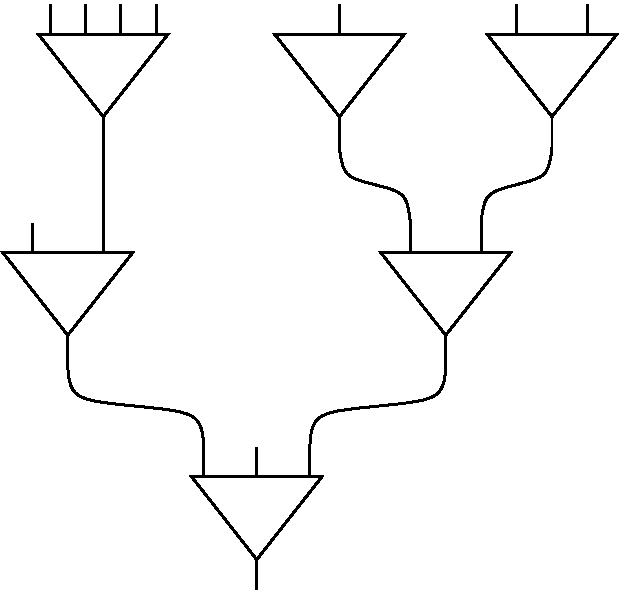
\includegraphics[height=60\unitlength]{transistor_bush2}}
\cell{55}{8}{c}{\normalsize$\theta$}
\cell{35.5}{31}{c}{\normalsize$\phi$}
\cell{74}{31}{c}{\normalsize$\psi$}
\cell{39}{53}{c}{\normalsize$\chi$}
\cell{63}{53}{c}{\normalsize$\xi$}
\cell{85}{53}{c}{\normalsize$\omega$}
\end{picture}
\caption{Every tree of operations in an operad $P$ has a well-defined
  composite (in this case, an element of $P_9$).}
\lbl{fig:opd-tree}
\end{figure}

\begin{examples}
\lbl{egs:opd}
\begin{enumerate}
\item 
There is an operad $\One$\ntn{termopd} in which $\One_n$ is the one-element
set for each $n \geq 0$.  The composition and identities are uniquely
determined.  With the obvious notion of map of operads, $\One$ is the
terminal%
% 
\index{operad!terminal}%
\index{terminal operad}
% 
operad.

\item
\lbl{eg:opd-M}
Fix a monoid%
%
\index{monoid!operad from}%
\index{operad!monoid@from monoid}
% 
$M$.  There is an operad $P(M)$\ntn{monopd} given by
\[
P(M)_n
=
\begin{cases}
M               &\text{if } n = 1,      \\
\emptyset       &\text{otherwise}
\end{cases}
\]
($n \geq 0$).  There is no choice in how to define the composition of
$P(M)$ except when $n = k_1 = 1$ (in the notation of~\eqref{eq:opd-comp}),
and in that case it is defined to be the multiplication of $M$.  Similarly,
the identity of the operad $P(M)$ is the identity of the monoid $M$.

\item
\lbl{eg:opd-Delta} 
% 
There is an operad%
%
\index{simplex!operad}%
\index{probability distribution!operad}%
\index{operad!simplex}
% 
\ntn{simpopd}$\Delta = (\Delta_n)_{n \geq 0}$, where as
usual $\Delta_n$ is the set of probability distributions on $\{1, \ldots,
n\}$.  The composition of the operad is composition of distributions,
% (Definition~\ref{defn:comp-dist}), 
and the identity is the unique distribution $\vc{u}_1$ on $\{1\}$.  We
already noted in Remark~\ref{rmk:comp-dist-opd} that the associativity and
identity axioms are satisfied.

\item
There is a larger operad $\measopd$ consisting of not just the
\emph{probability} measures on finite sets, but all finite measures%
%
\index{measure operad}%
\index{operad!measure}
% 
on finite sets.  Thus, $\measopd_n = [0, \infty)^n$.  The composition is
  given by the same formula as for $\Delta$
  (Definition~\ref{defn:comp-dist}), and the identity is $(1) \in
  \measopd_1$.

\item
\lbl{eg:opd-End}
Let $\cat{A}$ be a monoidal category and $A \in \cat{A}$. Then there is an
operad $\End(A)$%
%
\index{endomorphism operad}%
\index{operad!endomorphism} 
% 
with 
\[
\End(A)_n = \cat{A}(A^{\otimes n}, A),
\ntn{Endopd}
\]
and with composition and identities defined using the composition,
identities and monoidal structure of $\cat{A}$.  For a general operad $P$,
we have suggested that elements of $P_n$ be thought of as operations, but
when $P = \End(A)$, this is true in a concrete sense: $\End(A)_n$ is the set
of maps $A^{\otimes n} \to A$.

\item
Fix a field $k$, and let $P_n = k[x_1, \ldots, x_n]$ be the set of
polynomials%
%
\index{polynomial!operad}%
\index{operad!polynomial} 
% 
over $k$ in $n$ variables.  Then $P = (P_n)_{n \geq 0}$ has the
structure of an operad, with composition given by substitution and
reindexing of variable names.  For instance, if
\[
\theta = x_1^2 + x_2^3 \in P_2,
\quad
\phi = 2x_1 x_3 - x_2 \in P_3,
\quad
\psi = x_1 + x_2 x_3 x_4 \in P_4,
\]
then
\[
\theta \of (\phi, \psi)
=
(2x_1 x_3 - x_2)^2 + (x_4 + x_5 x_6 x_7)^3 \in P_7.
\]
This example of an operad is just one of a large family.  In this case,
$P_n$ is the free $k$-algebra on $n$ generators.  There are similar
examples where $P_n$ is the free group, free Lie algebra, free distributive
lattice, etc., on $n$ generators.  In all cases, composition is by
substitution and reindexing.

\item
\lbl{eg:opd-little-discs}
Fix $d \geq 1$.  The \demph{little%
%
\index{operad!little discs}%
\index{little discs operad} 
% 
$d$-discs operad} $P$ is defined as follows.  Let $P_n$ be the set of
configurations of $n$ $d$-dimensional discs inside the unit disc, numbered
in order and with disjoint interiors (Figure~\ref{fig:little-discs}).
% 
\begin{figure}
\centering
\lengths
\begin{picture}(54,58)
\cell{27}{30}{c}{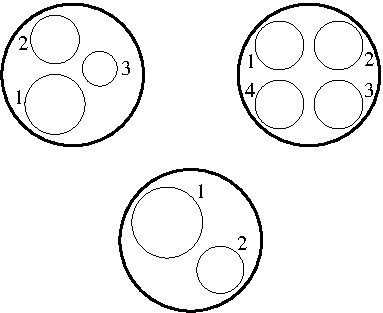
\includegraphics[width=54\unitlength]{discs_before}}
\cell{18}{9}{c}{\normalsize$\theta$}
\cell{3}{30}{c}{\normalsize$\phi$}
\cell{51}{30}{c}{\normalsize$\psi$}
% \cell{18}{27}{c}{\normalsize$\theta$}
% \cell{3}{52}{c}{\normalsize$\phi^1$}
% \cell{52}{52}{c}{\normalsize$\phi^2$}
\cell{27}{0}{b}{(a)}
\end{picture}%
\hspace*{12mm}%
\begin{picture}(54,58)
\cell{27}{34}{c}{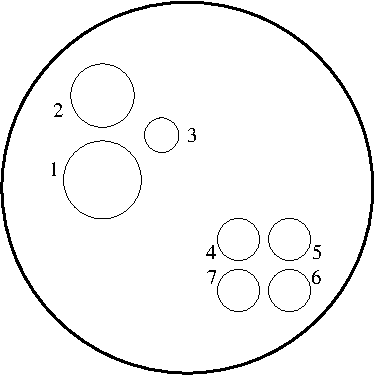
\includegraphics[width=48\unitlength]{discs_after}}
\cell{44}{8}{c}{\normalsize$\theta\of(\phi, \psi)$}
% \cell{10}{8}{c}{\normalsize$\theta\of(\phi^1, \phi^2)$}
% \cell{11}{55}{c}{\normalsize$\theta\of(\phi^1, \phi^2)$}
\cell{27}{0}{b}{(b)}
\end{picture}%
\caption{(a)~Operations $\theta \in P_2$, $\phi \in P_3$ and $\psi \in
P_4$ in the little $2$-discs operad $P$
(Example~\ref{egs:opd}\bref{eg:opd-little-discs}); (b)~the composite
operation $\theta \of (\phi, \psi) \in P_7$.}  
\lbl{fig:little-discs}
\end{figure}
% 
Composition is by substitution (using affine transformations) and
reindexing, as suggested by the figure.  

The little discs operad and its close relative, the little cubes operad,
were some of the very first operads to be defined (Boardman%
%
\index{Boardman, Michael} 
% 
and Vogt~\cite{BoVo}%
%
\index{Vogt, Rainer} 
% 
and Section~4 of May~\cite{MayGIL}).%
%
\index{May, J. Peter}
\end{enumerate}
\end{examples}

In more precise terminology, operads as defined in
Definition~\ref{defn:opd} are called nonsymmetric operads of sets.  Just as
the definition of monoidal category has symmetric and nonsymmetric
variants, so too does the definition of operad.  We will concentrate on the
nonsymmetric variant.

However, we will not only need operads \emph{of sets}.  Let $\cat{E}$ be
any category with finite products (or indeed, any symmetric monoidal
category, a level of generality that we will not need).  An \demph{operad%
%
\index{operad!internal} 
% 
in $\cat{E}$} is a sequence $(P_n)_{n \geq 0}$ of objects of $\cat{E}$
together with maps~\eqref{eq:opd-comp} in $\cat{E}$ (encoding the
composition) and a map $1 \to P_1$ in $\cat{E}$ (encoding the identity),
all subject to commutative diagrams expressing the associativity and
identity equations of Definition~\ref{defn:opd}.

Details of this more general definition can be found in May~\cite{MayDOA},
for instance, but we will need only two cases.  The first is $\cat{E} =
\Set$\ntn{Set}, the category of sets.  In that case, an operad in $\cat{E}$
is just an operad as in Definition~\ref{defn:opd}.  The second is $\cat{E}
= \Tp$\ntn{Tp}, the category of topological spaces.  An operad in $\Tp$ is
just an operad $P$ of sets in which each set $P_n$ is equipped with a
topology and the composition maps~\eqref{eq:opd-comp} are continuous. We
will refer to operads in $\Tp$ as \demph{topological%
% 
\index{topological operad} 
% 
operads}.

\begin{examples}
\begin{enumerate}
\item 
The terminal%
% 
\index{operad!terminal}%
\index{terminal operad}
% 
operad $\One$ is a topological operad in a unique way.

\item
For a topological monoid%
%
\index{monoid!operad from}%
\index{operad!monoid@from monoid}
% 
$M$, the operad $P(M)$ of Example~\ref{egs:opd}\bref{eg:opd-M} is a
topological operad in an evident way.

\item
Putting the standard topology on the simplices%
%
\index{simplex!operad}%
\index{probability distribution!operad}%
\index{operad!simplex}
% 
$\Delta_n$ gives $\Delta$
the structure of a topological operad.

\item
The little%
%
\index{operad!little discs}%
\index{little discs operad} 
% 
discs operad is also naturally a topological operad.
\end{enumerate}
\end{examples}

An operad $P$ is a system of abstract operations.  An algebra for $P$ is an
interpretation of the elements of $P$ as \emph{actual} operations:

\begin{defn}
\lbl{defn:alg}
Let $P$ be an operad of sets.  A \demph{$P$-algebra}%
%
\index{algebra for operad} 
% 
is a set $A$ together with a map
\[
\begin{array}{cccc}
\alpha_n \from  &P_n \times A^n &\to    &A      \\
&
\bigl(\theta, (a^1, \ldots, a^n)\bigr)  &\mapsto        &
\ovln{\theta}(a^1, \ldots, a^n)
\end{array}
\ntn{algbar}
\]
for each $n \geq 0$, satisfying two axioms:
% 
\begin{multline}
\lbl{eq:alg-comp}
\ovln{\theta \of (\phi^1, \ldots, \phi^n)}
\bigl(
a^{1 1}, \ldots, a^{1 k_1}, \ \ldots, \ a^{n 1}, \ldots, a^{n k_n}
\bigr)  \\
=
\ovln{\theta} \Bigl(
\ovln{\phi^1} \bigl( a^{1 1}, \ldots, a^{1 k_1} \bigr),
\ \ldots, \ 
\ovln{\phi^n} \bigl( a^{n 1}, \ldots, a^{n k_n} \bigr)
\Bigr)
\end{multline}
% 
for all $\theta \in P_n$, $\phi^i \in P_{k_i}$ and $a^{i j} \in A$; and
% 
\begin{equation}
\lbl{eq:alg-id}
\ovln{1_P}(a) = a
\end{equation}
% 
for all $a \in A$.
\end{defn}

The definition of algebra extends easily from operads of sets to operads in
any category $\cat{E}$ with finite products: then $A$ is an object of
$\cat{E}$ and $\alpha_n$ is a map in $\cat{E}$, while the
equations~\eqref{eq:alg-comp} and~\eqref{eq:alg-id} are expressed as
commutative diagrams in $\cat{E}$ (May~\cite{MayDOA}).  In the only other
case that concerns us here, $\cat{E} = \Tp$, an algebra%
%
\index{algebra for operad!topological}%
\index{topological operad!algebra for}
% 
for a topological operad $P$ is a topological space $A$ together with a
sequence of continuous maps
\[
\Bigl( P_n \times A^n \toby{\alpha_n} A \Bigr)_{n \geq 0}
\]
satisfying equations~\eqref{eq:alg-comp} and~\eqref{eq:alg-id}.

\begin{examples}
\lbl{egs:opd-alg}
\begin{enumerate}
\item
\lbl{eg:opd-alg-one} 
Consider the terminal%
% 
\index{operad!terminal}%
\index{terminal operad}
% 
operad $\One$ of sets.  A $\One$-algebra is a set $A$ together with a map
$\alpha_n \from A^n \to A$ for each $n \geq 0$, satisfying
equations~\eqref{eq:alg-comp} and~\eqref{eq:alg-id}.  One easily deduces
that a $\One$-algebra is exactly a monoid, with $\alpha_n$ as its $n$-fold
multiplication.  If $\One$ is regarded as a topological operad then a
$\One$-algebra is exactly a topological monoid.

\item
Fix a monoid%
%
\index{monoid!operad from}%
\index{operad!monoid@from monoid}
% 
$M$.  An algebra for the operad $P(M)$ is simply a set with a
left $M$-action.  If $M$ is a topological monoid then a $P(M)$-algebra is a
topological space with a continuous left $M$-action.

\item
\lbl{eg:opd-alg-simp}
Now consider the topological operad $\Delta$ of simplices.%
%
\index{simplex!operad}%
\index{probability distribution!operad}%
\index{operad!simplex}
% 
Any convex subset $A$ of $\R^d$, for any $d \geq 0$, is a $\Delta$-algebra
in a natural way: given $\p \in \Delta_n$ and $\vc{a}^1, \ldots, \vc{a}^n
\in A$, put
\[
\ovln{\p}(\vc{a}^1, \ldots, \vc{a}^n)
=
p_1 \vc{a}^1 + \cdots + p_n \vc{a}^n
\in 
A.
\]
Equations~\eqref{eq:alg-comp} and~\eqref{eq:alg-id} express elementary
facts about convex combinations.  

We refer to this as the \demph{standard}%
%
\index{standard Delta-algebra structure@standard $\Delta$-algebra structure} 
% 
$\Delta$-algebra structure on $A$.

\item
\lbl{eg:opd-alg-def}
The previous example admits a family of deformations,%
%
\index{deformed Delta-algebra structure@deformed $\Delta$-algebra structure} 
% 
at least when $A$ is a linear subspace of $\R^d$.  For each $q \in \R$,
there is a $\Delta$-algebra structure on $A$ given by
\[
\ovln{\p}(\vc{a}^1, \ldots, \vc{a}^n)
=
\sum_{i \in \supp{\p}} p_i^q \vc{a}^i.
\]
(Here the superscript $q$ is a power but the superscript $i$ is an
index.)  The previous example is the case $q = 1$.

\item
The chain%
%
\index{chain rule!means@for means} 
% 
rule for a weighted mean $M$ on an interval $I$ nearly states
that the maps
\[
\bigl(M \from \Delta_n \times I^n \to I\bigr)_{n \geq 0}
\]
give $I$ the structure of an algebra for the operad $\Delta$.  More
exactly, the chain rule is the composition axiom~\eqref{eq:alg-comp} for
a $\Delta$-algebra.  For $I$ to be a $\Delta$-algebra, it must also satisfy
the identity axiom~\eqref{eq:alg-id}, which is a special case of
consistency: $M(\vc{u}_1, (x)) = x$ for each $x \in I$.

\item
For any operad $P$ of sets, a $P$-algebra amounts to a set $A$ together
with a map $P \to \End(A)$ of operads.  Here, $\End(A)$%
%
\index{endomorphism operad}%
\index{operad!endomorphism} 
% 
is the operad defined in Example~\ref{egs:opd}\bref{eg:opd-End}, with
$\cat{A} = \Set$.  
% This makes precise the sentence preceding
% Definition~\ref{defn:alg}.
This makes precise the earlier assertion that an algebra for $P$ is an
interpretation of the elements of $P$ as actual operations.


\item
Any $d$-fold loop%
%
\index{loop space}
% 
space is an algebra for the little%
%
\index{operad!little discs}%
\index{little discs operad} 
% 
$d$-discs operad in a natural way.  This was one of the first examples of
an algebra for an operad, the details of which can be found in Section~5 of
May~\cite{MayGIL}.%
%
\index{May, J. Peter}
\end{enumerate}
\end{examples}

Let $P$ be an operad in a finite product category $\cat{E}$, and let $A =
(A, \alpha)$ and $B = (B, \beta)$ be $P$-algebras.  A \demph{map of
  $P$-algebras}%
%
\index{algebra for operad!map of} 
% 
from $A$ to $B$ is a map $f \from A \to B$ in $\cat{E}$
such that the square
\[
\xymatrix{
P_n \times A^n \ar[r]^{1 \times f^n} \ar[d]_{\alpha_n}  &
P_n \times B^n \ar[d]^{\beta_n} \\
A \ar[r]_{f}    &
B
}
\]
commutes for each $n \geq 0$.  This defines a category $\Alg(P)$\ntn{Alg}
of $P$-algebras.

\begin{remarks}
\lbl{rmks:opds-thys}
The language of operations and algebras invites comparison with other
categorical formulations of the concept of algebraic theory.  Systematic
comparisons can be found in Kelly~\cite{KellOOJ}, Section~2.8 of
Gould~\cite{GoulCCO}, and Chapter~3 of Avery~\cite{AverSS}.  Here, we just
make the following observations.
% 
\begin{enumerate}
\item 
\lbl{rmk:opds-thys-mnds}
Let $\cat{E}$ be a finite product category satisfying the further mild
condition that it has countable coproducts over which the product
distributes.  ($\Set$ and $\Tp$ are examples.)  Then any operad $P$ in
$\cat{E}$ induces a monad%
%
\index{operad!monad from}%
\index{monad!operad@from operad}
% 
$T_P$ on $\cat{E}$, with functor part given by
\[
T_P(A) = \coprod_{n \geq 0} P_n \times A^n
\]
($A \in \cat{E}$).  The category of algebras for the
operad $P$ is exactly the category of algebras for the monad $T_P$.
Non-isomorphic operads $P$ sometimes induce the same monad
$T_P$~\cite{AOAT}, although many aspects of an operad can still be
understood through its induced monad.

\item
\lbl{rmk:opds-thys-thys}
% Remark~\ref{rmks:opds-thys}
Remark~\bref{rmk:opds-thys-mnds} provides a semantic connection between
operads and a different conception of algebraic theory, monads.  On the
syntactic side, the definition of operad can easily be adapted to give a
definition of finitary algebraic theory, equivalent to any of the usual
definitions (as given in Manes~\cite{ManeAT}, for instance).  Indeed,
a finitary algebraic theory can be defined as an operad $P$ together with,
for each map of sets
\[
f \from \{1, \ldots, m\} \to \{1, \ldots, n\},
\]
a map $f_* \from P_m \to P_n$, subject to equations expressing
compatibility between the operad structure and these maps $f_*$
(Tronin~\cite{TronACO,TronOVA}).  The idea is that $f_*$ transforms an
$m$-ary operation into an $n$-ary operation by reindexing the variables
according to $f$.  For instance, in the theory $P$ of groups, $P_n$ is the
underlying set of the free group on $n$ generators (which can be regarded
as the set of $n$-ary operations defined on any group), and if $f$ is the
unique map $\{1, 2\} \to \{1\}$ then $f_*\from P_2 \to P_1$ sends the
operation of multiplication to the operation of squaring.

If we take the definition of finitary algebraic theory sketched in the
previous paragraph but restrict $f$ to be a bijection, we obtain the
definition of
\demph{symmetric%
%
\index{operad!symmetric}%
\index{symmetric!operad} 
% 
operad}.  (In much of the literature, `operad' is taken to mean `symmetric
operad' by default.)  If we further restrict $f$ to be an identity, we
recover the definition of nonsymmetric operad.

\item
As the previous remark suggests, most algebraic theories cannot be
described by an operad.  For instance, there is no operad $P$ of sets such
that $\Alg(P)$ is equivalent to the category of groups.%
%
\index{operad!groups@for groups, nonexistent}%
\index{groups, theory of}  
% 
For a proof of a strong version of this statement, see Lin~\cite{LinAGA}.
\end{enumerate}
\end{remarks}


\section{Categorical algebras and internal algebras}
\lbl{sec:cat-int-alg}


Let $P$ be an operad of sets.  An algebra for $P$ is a set acted on by $P$,
but more generally, we can consider \emph{categories} acted on by $P$.
Such a structure is called a categorical $P$-algebra.  

More generally still, let $\cat{E}$ be a category with finite limits.  Then
there is the notion of internal category in $\cat{E}$ (as in Chapter~2 of
Johnstone~\cite{JohnTT}), and when $P$ is an operad in
$\cat{E}$, we can consider actions of $P$ on such an internal category.

% The most concise way to state the definition is as follows.

\begin{defn}
\lbl{defn:cat-alg}
Let $\cat{E}$ be a category with finite limits and let $P$ be an operad in
$\cat{E}$.  A \demph{categorical%
%
\index{categorical algebra for operad} 
% 
$P$-algebra} is an internal category in $\Alg(P)$.
\end{defn}

It is straightforward to verify that $\Alg(P)$ has finite limits, computed
as in $\cat{E}$, so this definition does make sense.  But it is also
helpful to have at hand a more explicit form, as follows.

A categorical $P$-algebra $\scat{A}$ can be described as a
pair of ordinary $P$-algebras, $\scat{A}_0$\ntn{A0} and
$\scat{A}_1$\ntn{A1}, together with domain and codomain maps
\[
\scat{A}_1 \parpairu \scat{A}_0
\]
and composition and identity maps
\[
\scat{A}_1 \times_{\scat{A}_0} \scat{A}_1 \to \scat{A}_1,
\qquad
1 \to \scat{A}_1,
\]
all of which are required to be maps of $P$-algebras, as well as obeying
the usual axioms for an internal category.  Here $\scat{A}_0$ is to be
thought of as the object of objects of $\scat{A}$, and $\scat{A}_1$ as the
object of maps in $\scat{A}$.

Equivalently, a categorical $P$-algebra is an internal category in
$\cat{E}$ on which $P$ acts functorially.  To see this, first note that for
any object $X$ of $\cat{E}$ and internal category $\scat{A}$ in $\cat{E}$,
we can define another internal category
\[
X \times \scat{A}
\ntn{XA}
\]
in $\cat{E}$.  This is the product $D(X) \times \scat{A}$, where $D(X)$ is
the discrete internal category on $X$.  Thus, its object of objects
and object of maps are given by
\[
(X \times \scat{A})_0 = X \times \scat{A}_0,
\qquad
(X \times \scat{A})_1 = X \times \scat{A}_1.
\]
In this notation, a categorical $P$-algebra consists of an internal
category $\scat{A}$ in $\cat{E}$ together with internal functors
% 
\begin{equation}
\lbl{eq:int-ftr-act}
\alpha_n \from P_n \times \scat{A}^n \to \scat{A}
\end{equation}
% 
($n \geq 0$), satisfying analogues of the usual algebra axioms.  

% (For more on categorical algebras for an operad, see Section~3.4
% of~\cite{HOHC}, for instance.)

As usual, we are principally concerned with the cases $\cat{E} = \Set$ and
$\cat{E} = \Tp$, where categorical algebras for an operad can be
understood as follows.
% 
\begin{examples}
\lbl{egs:cat-alg-gen}
\begin{enumerate}
\item 
\lbl{eg:cat-alg-gen-set}
Let $P$ be an operad in $\cat{E} = \Set$.  A categorical $P$-algebra
consists of a small category $\scat{A}$ together with a functor
\[
\ovln{\theta} \from \scat{A}^n \to \scat{A}
\]
for each $n \geq 0$ and $\theta \in P_n$.  These functors are required to
satisfy equations~\eqref{eq:alg-comp} and~\eqref{eq:alg-id} for objects
$a^{ij}$ and $a$ of $\scat{A}$, and analogous equations for maps in
$\scat{A}$.

\item
\lbl{eg:cat-alg-gen-top}
Let $P$ be an operad%
%
\index{categorical algebra for operad!topological}%
\index{topological operad!categorical algebra for}
% 
in $\cat{E} = \Tp$.  The categorical $P$-algebras can be described as
in~\bref{eg:cat-alg-gen-set}, but with the following additions.  $\scat{A}$
is now a topological category, so that $\scat{A}_0$ and $\scat{A}_1$ carry
topologies with the property that the domain, codomain, composition and
identity operations are continuous.  Moreover, the structure maps
\[
P_n \times \scat{A}_0^n \to \scat{A}_0,
\quad
P_n \times \scat{A}_1^n \to \scat{A}_1
\]
of the $P$-algebras $\scat{A}_0$ and $\scat{A}_1$ are required to be
continuous. 

\item
\lbl{eg:cat-alg-gen-one} 
% 
Here we consider the special case of categorical algebras with only one%
%
\index{categorical algebra for operad!one-object} 
% 
object, over both $\Set$ and $\Tp$.

First, let $P$ be an operad of sets.  Let $A$ be a monoid, viewed as a
one-object category $\scat{A}$.  To give $\scat{A}$ the structure of a
categorical $P$-algebra is to give the set $A$ the structure of an ordinary
$P$-algebra in such a way that for each $n \geq 0$ and $\theta \in P_n$,
the structure map
\[
\ovln{\theta} \from A^n \to A
\]
is a monoid homomorphism.  In short, a one-object categorical $P$-algebra
is a monoid on which $P$ acts by homomorphisms.

Similarly, when $P$ is a topological operad, a one-object categorical
$P$-algebra is a topological monoid on which $P$ acts by continuous
homomorphisms. 
\end{enumerate}
\end{examples}

Some specific examples now follow.

\begin{examples}
\lbl{egs:cat-alg-spec}
\begin{enumerate}
\item 
Consider the terminal%
% 
\index{operad!terminal}%
\index{terminal operad}
% 
operad of sets, $\One$.  By the description preceding
equation~\eqref{eq:int-ftr-act}, a categorical $\One$-algebra is a category
on which $\One$ acts functorially, that is, a category $\scat{A}$ together
with a functor $\scat{A}^n \to \scat{A}$, subject to certain axioms.  These
axioms give $\scat{A}$ the structure of a monoid in $\Cat$.  Thus, a
categorical $\One$-algebra is exactly a strict monoidal category.

Alternatively, working directly from Definition~\ref{defn:cat-alg}, a
categorical $\One$-algebra is an internal category in $\Mon$, the category
of monoids.  Again, this is just a strict monoidal category.

\item
\lbl{eg:cat-alg-spec-act}
Let $M$ be a monoid,%
%
\index{monoid!operad from}%
\index{operad!monoid@from monoid}
% 
and form the operad $P(M)$ of sets (Example~\ref{egs:opd}\bref{eg:opd-M}).
A categorical $P(M)$-algebra is a category equipped with a left $M$-action.

\item
\lbl{eg:cat-alg-spec-simp}
Consider the topological operad $\Delta$%
%
\index{simplex!operad}%
\index{probability distribution!operad}%
\index{operad!simplex}
% 
of simplices.  Let $A$ be a linear subspace (or more generally, a convex
additive submonoid) of $\R^d$.  Then $A$ is a topological monoid under
addition.  We have already considered the standard%
%
\index{standard Delta-algebra structure@standard $\Delta$-algebra structure} 
%
$\Delta$-algebra structure on the topological space $A$, given for
$\p \in \Delta_n$ by
\[
\begin{array}{cccc}
\ovln{\p}\from  &
A^n                             &\to            &
A      \\
&
(\vc{a}^1, \ldots, \vc{a}^n)    &\mapsto        &
\sum_{i = 1}^n p_i \vc{a}^i
\end{array}
\]
(Example~\ref{egs:opd-alg}\bref{eg:opd-alg-simp}).  Each of these maps
$\ovln{\p}$ is a monoid homomorphism. Hence
by Example~\ref{egs:cat-alg-gen}\bref{eg:cat-alg-gen-one}, $A$ is a
one-object categorical $\Delta$-algebra.

\item
\lbl{eg:cat-alg-spec-def}
The same is true for the $q$-deformed%
%
\index{deformed Delta-algebra structure@deformed $\Delta$-algebra structure} 
%
algebra structure
\[
(\vc{a}^1, \ldots, \vc{a}^n)
\mapsto
\sum_{i \in \supp(\p)} p_i^q \vc{a}^i
\]
of Example~\ref{egs:opd-alg}\bref{eg:opd-alg-def}, for any $q \in \R$.  
\end{enumerate}
\end{examples}

For ordinary algebras for an operad, there is only one sensible notion of
map between algebras, but for \emph{categorical} algebras, there are
several.  Indeed, let $\cat{E}$ be a category with finite limits, let $P$
be an operad in $\cat{E}$, and let $\scat{B}$ and $\scat{A}$ be categorical
$P$-algebras.  Then $\scat{B}$ and $\scat{A}$ are, by definition, internal
categories in $\Alg(P)$, and a \demph{strict%
%
\index{strict map}%
\index{categorical algebra for operad!strict map of}
% 
map} from $\scat{B}$ to $\scat{A}$ is an internal functor $\scat{B} \to
\scat{A}$ in $\Alg(P)$.  Equivalently, it is an internal functor
\[
G \from \scat{B} \to \scat{A}
\]
in $\cat{E}$ such that for all $n \geq 0$, the square
\[
\xymatrix{
P_n \times \scat{B}^n \ar[r]^{1 \times G^n} \ar[d]_{\beta_n}  &
P_n \times \scat{A}^n \ar[d]^{\alpha_n} \\
\scat{B} \ar[r]_{G}    &
\scat{A}
}
\]
commutes, where $\beta_n$ and $\alpha_n$ are the structure maps of
$\scat{B}$ and $\scat{A}$ (as in equation~\eqref{eq:int-ftr-act}).

However, this is a square of (internal) categories and functors, so we can
also consider variants in which the square is only required to commute up
to a specified natural isomorphism, or a natural transformation in one
direction or the other~-- subject, as usual, to coherence axioms.  The
particular variant that will concern us is the following.

\begin{defn}
\lbl{defn:lax-map-cat-alg}
Let $\cat{E}$ be a category with finite limits and let $P$ be an operad in
$\cat{E}$.  Let $\scat{B}$ and $\scat{A}$ be categorical $P$-algebras, with
structure maps $(\beta_n)$ and $(\alpha_n)$ respectively.  A
\demph{lax%
%
\index{lax map}%
\index{categorical algebra for operad!lax map of}
% 
map} $\scat{B} \to \scat{A}$ of categorical $P$-algebras consists of a
functor $G \from \scat{B} \to \scat{A}$ (internal to $\cat{E}$) together
with a natural transformation
\[
\xymatrix{
P_n \times \scat{B}^n 
\ar[r]^{1 \times G^n} \ar[d]_{\beta_n} \ar@{}[dr]|-{\swnt\gamma_n}      &
P_n \times \scat{A}^n \ar[d]^{\alpha_n} \\
\scat{B} \ar[r]_G       &
\scat{A}
}
\]
(again internal to $\cat{E}$) for each $n \geq 0$, satisfying the following
two axioms:
% 
\begin{enumerate}
\item 
For each $n, k_1, \ldots, k_n \geq 0$, writing $k = \sum k_i$, 
the composite natural transformation
% 
\[
\xymatrix@C+6em{
\diagstack{P_n \times P_{k_1} \times \scat{B}^{k_1} \times \cdots 
\hspace*{8mm}}%
{\hspace*{20mm}{}\times P_{k_n} \times \scat{B}^{k_n}}
\ar@{}[dr]|-{\swnt 1 \times \gamma_{k_1} \times \cdots \times \gamma_{k_n}}
\ar[d]_{1 \times \beta_{k_1} \times \cdots \times \beta_{k_n}} 
\ar[r]^{1 \times 1 \times G^{k_1} \times \cdots \times 1 \times G^{k_n}}
&
\diagstack{P_n \times P_{k_1} \times \scat{A}^{k_1} \times \cdots
\hspace*{8mm}}% 
{\hspace*{20mm}{}\times P_{k_n} \times \scat{A}^{k_n}}
\ar[d]^{1 \times \alpha_{k_1} \times \cdots \times \alpha_{k_n}}   \\
P_n \times \scat{B}^n
\ar@{}[dr]|-{\swnt \gamma_n}
\ar[d]_{\beta_n}
\ar[r]|{\:1 \times G^n\:}       &
P_n \times \scat{A}^n   
\ar[d]^{\alpha_n}        \\
\scat{B} \ar[r]_G       &
\scat{A}
}
\]
is equal to 
\[
\xymatrix@C+6em{
\diagstack{P_n \times P_{k_1} \times \scat{B}^{k_1} \times \cdots
\hspace*{8mm}}%
{\hspace*{20mm}{}\times P_{k_n} \times \scat{B}^{k_n}}
\ar[d]_{\iso} 
\ar[r]^{1 \times 1 \times G^{k_1} \times \cdots \times 1 \times G^{k_n}}
&
\diagstack{P_n \times P_{k_1} \times \scat{A}^{k_1} \times \cdots
\hspace*{8mm}}% 
{\hspace*{20mm}{} \times P_{k_n} \times \scat{A}^{k_n}}
\ar[d]^{\iso}   \\
P_n \times P_{k_1} \times \cdots \times P_{k_n} \times \scat{B}^k
\ar[d]_{\of \times 1}
\ar@{}[r]|-{\neeq} &
P_n \times P_{k_1} \times \cdots \times P_{k_n} \times \scat{A}^k       
\ar[d]^{\of \times 1}   \\
P_k \times \scat{B}^k
\ar@{}[dr]|-{\swnt \gamma_k}
\ar[d]_{\beta_k}
\ar[r]|{\:1 \times G^k\:}   &
P_k \times \scat{A}^k   
\ar[d]^{\alpha_k}        \\
\scat{B} \ar[r]_G       &
\scat{A}.
}
\]

\item
The composite natural transformation
\[
\xymatrix@C+3em{
\scat{B} \ar[d]_{\iso} \ar[r]^G &
\scat{A} \ar[d]^{\iso}  \\
1 \times \scat{B} \ar[d]_{1_P \times 1} \ar@{}[r]|-{\neeq}      &
1 \times \scat{A} \ar[d]^{1_P \times 1} \\
P_1 \times \scat{B} 
\ar@{}[dr]|-{\swnt \gamma_1} 
\ar[d]_{\beta_1} 
\ar[r]|{\:1 \times G\:} &
P_1 \times \scat{A} \ar[d]^{\alpha_1}   \\
\scat{B} \ar[r]_G       &
\scat{A}
}
\]
is equal to the identity.  (Here, $1_P \from 1 \to P_1$ denotes the map
encoding the identity of the operad $P$.)
\end{enumerate}
\end{defn}

A strict map of $P$-algebras can equivalently be viewed as a lax map $(G,
\gamma)$ in which each of the maps $\gamma_n$ is an identity.

\begin{remark}
Definition~\ref{defn:lax-map-cat-alg} can also be derived from the theory
of 2-monads,% 
%
\index{monad!two-@2-}%
\index{two-monad@2-monad}%
\index{operad!two-monad from@2-monad from} 
% 
as follows.  We observed in
Remark~\ref{rmks:opds-thys}\bref{rmk:opds-thys-mnds} that any operad $P$ in
$\cat{E}$ induces a monad $T_P$ on $\cat{E}$ (under mild hypotheses on the
category $\cat{E}$).  In the same way, it induces a 2-monad on
$\Cat(\cat{E})$, the 2-category of internal categories in $\cat{E}$.  An
algebra for that 2-monad is exactly a categorical $P$-algebra, and a lax
map of algebras for the 2-monad (in the sense of Blackwell, Kelly and
Power~\cite{BKP}) is exactly a lax map of categorical $P$-algebras.
\end{remark}

As a general categorical principle, it is often worth considering the maps
into an object from the terminal object.  (In categories of spaces, this
gives the notion of point.)  For any operad $P$ in any category $\cat{E}$
with finite limits, there is a terminal categorical $P$-algebra $\One$.  We
consider the lax maps from $\One$ to other categorical $P$-algebras.

\begin{defn}
\lbl{defn:int-alg}
Let $\cat{E}$ be a category with finite limits, let $P$ be an operad in
$\cat{E}$, and let $\scat{A}$ be a categorical $P$-algebra.  An
\demph{internal%
%
\index{internal algebra}%
\index{categorical algebra for operad!internal algebra in}
% 
algebra} in $\scat{A}$ is a lax map $\One \to \scat{A}$ of categorical
$P$-algebras.
\end{defn}

This definition is due to Batanin%
% 
\index{Batanin, Michael}  
% 
(\cite{BataEHA}, Definition~7.2).  We will see that it generalizes the
notion of internal monoid in a monoidal category.  But first, we give an
explicit description of internal algebras in the cases $\cat{E} = \Set$ and
$\cat{E} = \Tp$.

\begin{examples}
\lbl{egs:int-alg-gen}
\begin{enumerate}
\item 
\lbl{eg:int-alg-gen-Set}
Let $\cat{E} = \Set$.  Take an operad $P$ of sets and a categorical
$P$-algebra $\scat{A}$.  An internal algebra in $\scat{A}$ consists of, first
of all, a functor $G \from \One \to \scat{A}$.  This simply picks out an
object $a$ of $\scat{A}$.  Next, the natural transformations $\gamma_n$ in
Definition~\ref{defn:lax-map-cat-alg} amount to a family of
maps 
\[
\gamma_\theta \from 
\ovln{\theta}(\underbrace{a, \ldots, a}_n)
\to 
a,
\]
one for each $n \geq 0$ and $\theta \in P_n$.  The first coherence axiom in
Definition~\ref{defn:lax-map-cat-alg} states that the diagram
\[
\xymatrix@C+4em{
\ovln{\theta}\Bigl( 
\ovln{\phi^1}(a, \ldots, a), \ldots, \ovln{\phi^n}(a, \ldots, a)
\Bigr)
\ar[r]^-{\ovln{\theta}(\gamma_{\phi^1}, \ldots, \gamma_{\phi^n})}
\ar@{=}[d]      &
\ovln{\theta}(a, \ldots, a)
\ar[d]^{\gamma_\theta}  \\
\ovln{\theta \of (\phi^1, \ldots, \phi^n)}(a, \ldots, a)
\ar[r]_-{\gamma_{\theta \of (\phi^1, \ldots, \phi^n)}}  &
a
}
\]
commutes for all $\theta \in P_n$ and $\phi^i \in P_{k_i}$, and the second
states that
\[
\gamma_{1_P} \from \ovln{1_P}(a) \to a
\]
is equal to the identity on $a$.

\item
An identical description of internal algebras applies when $\cat{E} = \Tp$,
with the additional condition that for each $n \geq 0$, the function
\[
\begin{array}{ccc}
P_n     &\to            &\scat{A}_1     \\
\theta  &\mapsto        &\gamma_\theta
\end{array}
\]
is continuous.  (Here $\scat{A}_1$ denotes the space of maps in
the topological category $\scat{A}$, as in
Example~\ref{egs:cat-alg-gen}\bref{eg:cat-alg-gen-top}.) 

\item
\lbl{eg:int-alg-gen-mon}
Now let $\cat{E} = \Set$, and let $\scat{A}$ be a one-object%
%
\index{categorical algebra for operad!one-object}
% 
categorical $P$-algebra.  As we saw in
Example~\ref{egs:cat-alg-gen}\bref{eg:cat-alg-gen-one}, $\scat{A}$ amounts
to a monoid $A$ on which $P$ acts by homomorphisms.  An internal
$P$-algebra in $\scat{A}$ consists of an element $\gamma_\theta \in A$ for
each $n \geq 0$ and $\theta \in P_n$, satisfying the coherence axioms
in~\bref{eg:int-alg-gen-Set}. 

Writing $\gamma_\theta$ as $\gamma(\theta)$, we have a sequence of
functions
\[
\bigl( \gamma \from P_n \to A \bigr)_{n \geq 0}.
\]
The coherence axioms in~\bref{eg:int-alg-gen-Set} state that 
% 
\begin{equation}
\lbl{eq:iagm-1}
\gamma(\theta) \cdot 
\ovln{\theta}\bigl(\gamma(\phi^1), \ldots, \gamma(\phi^n)\bigr)
=
\gamma\bigl(\theta \of (\phi^1, \ldots, \phi^n)\bigr)
\end{equation}
% 
for all $n, k_1, \ldots, k_n \geq 0$, $\theta \in P_n$ and $\phi^i \in
P_{k_i}$, and that
% 
\begin{equation}
\lbl{eq:iagm-2}
\gamma(1_P) = 1.
\end{equation}
% 
In summary, when $\scat{A}$ is a one-object categorical $P$-algebra
corresponding to a monoid $A$, an internal $P$-algebra in $\scat{A}$
amounts to a sequence of maps $\gamma \from P_n \to A$ satisfying
equations~\eqref{eq:iagm-1} and~\eqref{eq:iagm-2}.

\item
\lbl{eg:int-alg-gen-top-mon}
For a topological operad $P$, internal algebras in a one-object categorical
$P$-algebra admit exactly the same explicit description as in the previous
example, with the added requirement that the maps $\gamma \from P_n \to A$
are continuous.
\end{enumerate}
\end{examples}

We now give some specific examples.

\begin{examples}
\lbl{egs:int-alg}
\begin{enumerate}
\item
Let $\One$ be the terminal%
% 
\index{operad!terminal}%
\index{terminal operad}
% 
operad of sets.  As we have seen, a categorical
$\One$-algebra is just a monoidal category.  By the explicit
description in Example~\ref{egs:int-alg-gen}\bref{eg:int-alg-gen-Set}, an
internal algebra in a categorical $\One$-algebra $\scat{A}$ consists
of an object $a \in \scat{A}$ together with a map 
\[
\gamma_n \from a^{\otimes n} \to a
\]
for each $n \geq 0$, satisfying the equations given there.  It follows
easily that an internal algebra in $\scat{A}$ is exactly a monoid%
%
\index{monoid!monoidal category@in monoidal category}
% 
in the monoidal category $\scat{A}$.

As an alternative proof, note that for strict monoidal
categories $\scat{B}$ and $\scat{A}$, a lax map $\scat{B} \to \scat{A}$ of
categorical $\One$-algebras is precisely a lax monoidal functor.  This is
immediate from the definitions.  Hence an internal algebra in a strict
monoidal category $\scat{A}$ is a lax monoidal functor $\One \to \scat{A}$,
and it is well-known that such functors correspond naturally to monoids in
$\scat{A}$ (paragraph~(5.4.1) of B\'enabou~\cite{BenIB}).

An algebra for $\One$ is exactly a monoid
(Example~\ref{egs:opd-alg}\bref{eg:opd-alg-one}), so it is logical
terminology that an internal algebra is exactly an internal monoid.

\item
Fix a monoid%
%
\index{monoid!operad from}%
\index{operad!monoid@from monoid}
% 
$M$.  We saw in Example~\ref{egs:cat-alg-spec}\bref{eg:cat-alg-spec-act}
that a categorical $P(M)$-algebra is a category $\scat{A}$ with a left
$M$-action; let us write the action as
\[
\begin{array}{ccc}
M \times \scat{A}       &\to            &\scat{A}       \\
(m, a)                  &\mapsto        &m \cdot a.
\end{array}
\]
By the explicit description in
Example~\ref{egs:int-alg-gen}\bref{eg:int-alg-gen-Set}, an internal
$P(M)$-algebra in $\scat{A}$ consists of an object $a \in \scat{A}$
together with a map
\[
\gamma_m \from m \cdot a \to a
\]
for each $m \in M$, satisfying natural coherence axioms.  
\end{enumerate}
\end{examples}

Missing from this list of examples is the case of internal algebras in a
categorical algebra for $\Delta$, the operad of simplices.  This is the
subject of the next section, and will transport us directly to the concept
of entropy.


\section{Entropy as an internal algebra}
\lbl{sec:cat-ent}
\index{entropy!internal algebra@as internal algebra}
\index{internal algebra!entropy as}


In this chapter so far, we have reviewed some established general
concepts in the theory of operads.  We now apply them to the topological
operad $\Delta$ of simplices.

We saw in Example~\ref{egs:cat-alg-spec}\bref{eg:cat-alg-spec-simp} that
the real line $\R$, as a topological monoid under addition, is a
categorical $\Delta$-algebra in a standard way:
% 
\begin{equation}
\lbl{eq:R-cat-alg}
\bigl(\p, (x_1, \ldots, x_n)\bigr) \mapsto \sum_{i = 1}^n p_i x_i
\end{equation}
% 
($\p \in \Delta_n$, $x_1, \ldots, x_n \in \R$).  What are the internal
algebras in the categorical $\Delta$-algebra $\R$?

By Example~\ref{egs:int-alg-gen}\bref{eg:int-alg-gen-top-mon}, an internal
$\Delta$-algebra in $\R$ amounts to a sequence of functions $\bigl( \gamma
\from \Delta_n \to \R \bigr)_{n \geq 0}$ satisfying certain axioms.  It is
in this sense that the following theorem holds.

\begin{thm}
\lbl{thm:cat-ent}%
\index{R@$\R$, internal algebras in}
% 
Let $\Delta$ be the topological operad of simplices, and equip $\R$ with
its standard%
%
\index{standard Delta-algebra structure@standard $\Delta$-algebra structure} 
%
categorical $\Delta$-algebra structure~\eqref{eq:R-cat-alg}.
Then the internal algebras in $\R$ are precisely the real scalar multiples
of Shannon entropy.
\end{thm}

In other words, a sequence of functions $\bigl( \gamma \from \Delta_n \to
\R \bigr)_{n \geq 0}$ defines an internal algebra in $\R$ if and only if
$\gamma = cH$ for some $c \in \R$.

\begin{proof}
By Example~\ref{egs:int-alg-gen}\bref{eg:int-alg-gen-top-mon}, an internal
algebra in $\R$ is a sequence of functions $\bigl( \gamma \from \Delta_n
\to \R \bigr)_{n \geq 0}$ with the following properties:
% 
\begin{enumerate}
\item 
\lbl{part:cat-ent-chain}
for all $n, k_1, \ldots, k_n \geq 0$ and $\vc{w} \in \Delta_n$, $\p^1
\in \Delta_{k_1}, \ldots, \p^n \in \Delta_{k_n}$,
\[
\gamma(\vc{w}) + \sum_{i = 1}^n w_i \gamma(\p^i)
=
\gamma\bigl(\vc{w} \of (\p^1, \ldots, \p^n)\bigr);
\]

\item
\lbl{part:cat-ent-unit}
$\gamma(\vc{u}_1) = 0$;

\item
$\gamma \from \Delta_n \to \R$ is continuous for each $n \geq 0$.
\end{enumerate}
% 
Condition~\bref{part:cat-ent-unit} is redundant, since it follows
from~\bref{part:cat-ent-chain} by taking $n = k_1 = 1$ and $\vc{w} = \p^1 =
\vc{u}_1$.  Hence by Faddeev's Theorem~\ref{thm:faddeev}, $\gamma$ defines
an internal algebra if and only if $\gamma = cH$ for some $c \in \R$.
\end{proof}

This theorem can be deformed.%
%
\index{deformed Delta-algebra structure@deformed $\Delta$-algebra structure} 
%
In Example~\ref{egs:cat-alg-spec}\bref{eg:cat-alg-spec-def}, we defined 
a one-parameter family of categorical $\Delta$-algebra structures
on $\R$, where for a real parameter $q$, the action of $\Delta$ on
$\R$ is 
% 
\begin{equation}
\lbl{eq:R-q-cat-alg}
\bigl(\p, (x_1, \ldots, x_n)\bigr) 
\mapsto 
\sum_{i \in \supp(\p)} p_i^q x_i
\end{equation}
% 
($\p \in \Delta_n$, $x_1, \ldots, x_n \in \R$).  

\begin{thm}
\lbl{thm:q-cat-ent}%
\index{R@$\R$, internal algebras in}
% 
Let $1 \neq q \in \R$.  Let $\Delta$ be the operad of simplices, considered
as an operad of sets, and equip $\R$ with its $q$-deformed categorical
$\Delta$-algebra structure~\eqref{eq:R-q-cat-alg}.  Then the internal
algebras in $\R$ are precisely the real scalar multiples of $q$-logarithmic
entropy.%
%
\index{internal algebra!q-logarithmic entropy as@$q$-logarithmic entropy as}
\index{q-logarithmic entropy@$q$-logarithmic entropy!internal algebra@as internal algebra}
\end{thm}

\begin{proof}
By Example~\ref{egs:int-alg-gen}\bref{eg:int-alg-gen-mon}, an internal
algebra in $\R$ is a sequence of functions $\bigl( \gamma \from \Delta_n
\to \R \bigr)_{n \geq 0}$ with the following properties:
% 
\begin{enumerate}
\item 
\lbl{part:q-cat-ent-chain}
for all $n, k_1, \ldots, k_n \geq 0$ and all $\vc{w} \in \Delta_n$, $\p^1
\in \Delta_{k_1}, \ldots, \p^n \in \Delta_{k_n}$,
\[
\gamma(\vc{w}) + \sum_{i \in \supp(\vc{w})} w_i^q \gamma(\p^i)
=
\gamma\bigl(\vc{w} \of (\p^1, \ldots, \p^n)\bigr);
\]

\item
\lbl{part:q-cat-ent-unit}
$\gamma(\vc{u}_1) = 0$.
\end{enumerate}
% 
Condition~\bref{part:q-cat-ent-unit} is redundant, for the same reason as
in the proof of Theorem~\ref{thm:cat-ent}.
Condition~\bref{part:q-cat-ent-chain} is satisfied if $\gamma = cS_q$, by
the chain rule~\eqref{eq:q-ent-chain} for $q$-logarithmic entropies.
Conversely, condition~\bref{part:q-cat-ent-chain} implies that
\[
\gamma(\vc{w} \otimes \p) 
= 
\gamma(\vc{w}) + 
\Biggl(\sum_{i \in \supp(\vc{w})} w_i^q\Biggr) \gamma(\vc{p})
\]
for all $\vc{w} \in \Delta_n$ and $\p \in \Delta_k$, by taking $\p^1 =
\cdots = \p^n = \p$.  Hence by Theorem~\ref{thm:q-ent-char}, if $\gamma$
defines an internal algebra then $\gamma = cS_q$ for some $c \in
\R$.
\end{proof}

Continuity was not needed in this theorem, and in fact the structure maps
$\Delta_n \times \R^n \to \R$ of the $q$-deformed $\Delta$-algebra $\R$ are
discontinuous when $q \leq 0$.  But they are evidently continuous when $q >
0$, so we have:

\begin{cor}
Let $q \in (0, \infty)$.  Let $\Delta$ be the topological operad of
simplices, and equip $\R$ with its $q$-deformed categorical
$\Delta$-algebra structure~\eqref{eq:R-q-cat-alg}.  Then the internal
algebras in $\R$ are precisely the real scalar multiples of $q$-logarithmic
entropy. 
\end{cor}

\begin{proof}
The case $q = 1$ is Theorem~\ref{thm:cat-ent}, and all other cases
follow from Theorem~\ref{thm:q-cat-ent}.
\end{proof}


\section{The universal internal algebra}
\lbl{sec:univ-int}
\index{internal algebra!universal}
\index{universal internal algebra}
\index{universal property}


In algebra, an important role is played by free algebraic structures
(groups, modules, etc.).  But since one forms the free algebraic structure
on a \emph{set}, and a set is merely a cardinality (for these purposes at
least), the possibilities are in a sense limited.  Greater riches are to be
found one categorical level up, where one can speak of the free categorical
structure containing some specified internal algebraic structure.  This
leads to categorical characterizations of some important
mathematical objects.
% 
\begin{examples}
\begin{enumerate}
\item 
The free monoidal category containing a monoid%
% 
\index{monoid!monoidal category@in monoidal category} 
% 
is equivalent to the
category of finite totally ordered%
%
\index{order!finite total}
% 
sets (Mac~Lane~\cite{MacLCWM}, Proposition~VII.5.1).  We will return to
this example shortly.  Informally, the statement is that if we build a
monoidal category by starting from nothing, putting in an internal monoid,
then adjoining no more other objects and maps than are forced by the
definitions, and making no unnecessary identifications, then the result is
the category of finite totally ordered sets.

\item
The free monoidal category containing an object $A$ and an isomorphism $A
\otimes A \to A$ is equivalent to the disjoint union of the terminal
category and Thompson's%
%
\index{Thompson's group $F$} 
% 
group $F$, viewed as a one-object category (Fiore%
%
\index{Fiore, Marcelo}
%  
and Leinster~\cite{ACTGF}).  

(Thompson's group is an infinite group with remarkable properties; it
has been rediscovered multiple times in diverse contexts.  Cannon, Floyd and
Parry~\cite{CFP} provide a survey.  A major open question, which
has attracted an exceptional number of opposing claims and retractions, is
whether $F$ is amenable.  Cannon and Floyd~\cite{CaFl} report that even
among experts, opinion is evenly split.)

\item
The free symmetric monoidal category containing a commutative Frobenius
algebra is the category of compact oriented 1-manifolds and 2-dimensional
cobordisms between them (Theorem~3.6.19 of Kock~\cite{KockFA2}, for
instance).  This result lies at the foundations of topological%
%
\index{topological quantum field theory} 
% 
quantum field theory.

\item
The free finite product category containing a group is the
Lawvere%
%
\index{Lawvere, F. William!theory} 
% 
theory of groups.  The same statement holds for any other algebraic
structure in place of groups (Lawvere~\cite{LawvFSA}).  This is essentially
a tautology, but expresses a fundamental insight of categorical universal
algebra: an algebraic theory can be understood as a finite product
category, and a model of a theory as a finite-product-preserving functor.
\end{enumerate}
\end{examples}

In this section, we construct the free categorical $P$-algebra containing
an internal algebra, where $P$ is any given operad.  We proceed as follows.
First, we construct a certain categorical $P$-algebra $FP$.  Then, we make
precise what it means for a categorical $P$-algebra to be `free containing
an internal algebra'.  Next, we prove that $FP$ has that property.  This
last result, applied in the case $P = \Delta$, leads to a characterization
of information loss.

We begin by constructing the categorical $P$-algebra $FP$\ntn{freecat}, for
an operad $P$ of sets.

The objects of $FP$ are the pairs $(n, \theta)$ with $n \geq 0$ and $\theta
\in P_n$.  Where confusion will not arise, we write $(n, \theta)$ as just
$\theta$.  For objects $\psi = (k, \psi)$ and $\theta = (n, \theta)$, a map
$\psi \to \theta$ in $FP$ consists of integers $k_1, \ldots, k_n \geq 0$
and operations $\phi^1 \in P_{k_1}, \ldots, \phi^n \in P_{k_n}$ such that
\[
k = k_1 + \cdots + k_n, 
\qquad
\psi = \theta \of (\phi^1, \ldots, \phi^n).
\]
We write this map as
% 
\begin{equation}
\lbl{eq:typical-FP-map}
\Fmap{\phi^1, \ldots, \phi^n}{\theta} \from \psi \to \theta.
\end{equation}
% 
Thus, the set of objects of the category $FP$ and the set of maps in $FP$
are, respectively,
% 
\begin{equation}
\lbl{eq:FP-oa}
\coprod_{n \geq 0} P_n,
\qquad
\coprod_{n, k_1, \ldots, k_n \geq 0} 
P_n \times P_{k_1} \times \cdots \times P_{k_n}.
\end{equation}
% 
Composition and identities in the category $FP$ are defined using the
composition and identity of the operad $P$.

To give the category $FP$ the structure of a categorical $P$-algebra, we
must construct from each operation $\pi \in P_m$ a functor
\[
\ovln{\pi}\from (FP)^m \to FP.
\]
On objects, $\ovln{\pi}$ is defined by
\[
\ovln{\pi} (\theta^1, \ldots, \theta^m)
=
\pi \of (\theta^1, \ldots, \theta^m).
\]
To define the action of $\ovln{\pi}$ on maps, take an $m$-tuple of maps 
% 
\begin{align*}
\Fmap{\phi^{1 1}, \ldots, \phi^{1 n_1}}{\theta^1} \from       &
\psi^1 \to \theta^1    \\
\vdots  \\
\Fmap{\phi^{m 1}, \ldots, \phi^{m n_m}}{\theta^m} \from       &
\psi^m \to \theta^m
\end{align*}
% 
in $FP$.  Then
% 
\begin{multline}
\lbl{eq:FP-act-maps} 
\ovln{\pi}\Bigl(
\Fmap{\phi^{1 1}, \ldots, \phi^{1 n_1}}{\theta^1},
\ \ldots, \ 
\Fmap{\phi^{m 1}, \ldots, \phi^{m n_m}}{\theta^m}
\Bigr)  \\
=
\Fmap{\phi^{1 1}, \ldots, \phi^{1 n_1},
\ \ldots, \
\phi^{m 1}, \ldots, \phi^{m n_m}}%
{\pi\of(\theta^1, \ldots, \theta^m)},
\end{multline}
% 
which is a map $\ovln{\pi}(\psi^1, \ldots, \psi^m) \to
\ovln{\pi}(\theta^1, \ldots, \theta^m)$ in $FP$. 

Verifying that $FP$
satisfies the axioms for a categorical $P$-algebra is routine.

% We pause to note two features of the categorical $P$-algebra $FP$.

\begin{lemma}
\lbl{lemma:FP-term}
Let $P$ be an operad of sets.  
% 
\begin{enumerate}
\item 
\lbl{part:FP-term-term}
The object $1_P$ of $FP$ is terminal.

\item
\lbl{part:FP-term-decomp}
% 
Write $\uqq{\phi}\ntn{toterm} \from \phi \to 1_P$ for the unique map from
an object $\phi$ of $FP$ to $1_P$.  Then for any map
\[
\Fmap{\phi^1, \ldots, \phi^n}{\theta} \from \psi \to \theta
\]
in $FP$, we have
\[
\Fmap{\phi^1, \ldots, \phi^n}{\theta}
=
\ovln{\theta}(\uqq{\phi^1}, \ldots, \uqq{\phi_n}).
\]
\end{enumerate}
\end{lemma}

The notation in~\bref{part:FP-term-term} refers to the identity element
$1_P \in P_1$ of the operad $P$, which corresponds to the object
$1_P\ntn{idopdobj} = (1, 1_P)$ of the category $FP$.  It is this object
that is terminal.

\begin{proof}
For~\bref{part:FP-term-term}, given any object $\phi$ of $FP$, it is
immediate from the definition of $FP$ that there is a unique map $\phi \to
1_P$, namely, 
\[
\uqq{\phi} = \Fmap{\phi}{1_P} \from \phi \to 1_P.
\]

For~\bref{part:FP-term-decomp}, take a map
\[
\Fmap{\phi^1, \ldots, \phi^n}{\theta} \from \psi \to \theta
\]
in $FP$.  Since $\uqq{\phi^i}$ is a map $\phi^i \to 1_P$, the map
$
\ovln{\theta}(\uqq{\phi^1}, \ldots, \uqq{\phi_n})
$
has domain 
\[
\ovln{\theta}(\phi^1, \ldots, \phi^n)
=
\theta \of (\phi^1, \ldots, \phi^n)
=
\psi
\]
and codomain
\[
\ovln{\theta}(1_P, \ldots, 1_P)
=
\theta \of (1_P, \ldots, 1_P)
=
\theta,
\]
matching the domain and codomain of $\Fmap{\phi^1, \ldots,
  \phi^n}{\theta}$.  Now by definition of $\uqq{\phi^i}$ and by
definition~\eqref{eq:FP-act-maps} of the $P$-action on maps in $FP$,
% 
\begin{align*}
\ovln{\theta}(\uqq{\phi^1}, \ldots, \uqq{\phi_n})   &
=
\ovln{\theta}\bigl(\Fmap{\phi^1}{1_P}, \ldots, \Fmap{\phi^n}{1_P}\bigr) \\
&
=
\Fmap{\phi^1, \ldots, \phi^n}{\theta\of(1_P, \ldots, 1_P)}      \\
&
=
\Fmap{\phi^1, \ldots, \phi^n}{\theta},
\end{align*}
% 
as required.
\end{proof}

The categorical $P$-algebra $FP$ contains a canonical internal algebra.  To
specify it, we use the description of internal algebras in
Example~\ref{egs:int-alg-gen}\bref{eg:int-alg-gen-Set}.  Its underlying
object is the terminal object $1_P$.  To give $1_P$ the structure of an
internal algebra, we have to specify, for each $n \geq 0$ and $\theta \in
P_n$, a map
\[
\ovln{\theta}
\bigl(\,
\underbrace{1_P, \ldots, 1_P}_n
\,\bigr)
\to 
1_P.
\]
The domain here is $\theta$, and the codomain is terminal, so the only
possible choice is the unique map $\uqq{\theta} \from \theta \to 1_P$.
This gives $1_P$ the structure of an internal algebra in the categorical
$P$-algebra $FP$.  We refer to this internal algebra as $(1_P, !)$.

When $P$ is a topological operad, the set of objects of $FP$ and the set of
maps in $FP$ (both given in~\eqref{eq:FP-oa}) each carry a natural
topology.  For instance, the set of maps in $FP$ is a coproduct of product
spaces.  In this way, $FP$ is an internal category in $\Tp$.
Indeed, $FP$ is a categorical $P$-algebra in the topological sense (by the
description in Example~\ref{egs:cat-alg-gen}\bref{eg:cat-alg-gen-top}) and
$(1_P, !)$ is an internal algebra in $FP$ in the topological sense (by the
description in Example~\ref{egs:int-alg-gen}\bref{eg:int-alg-gen-top-mon}.)

\begin{remark}
As for all of the operadic definitions and constructions in this chapter,
the construction of $FP$ can be generalized to an operad $P$ in an
arbitrary category $\cat{E}$ with suitable properties (in this case, finite
products and countable coproducts over which the products distribute).  The
general definition is exactly as suggested by the case $\cat{E} = \Tp$.
\end{remark}

\begin{examples}
\lbl{egs:F}
\begin{enumerate}
\item 
\lbl{eg:F-mon}
Consider the terminal%
% 
\index{operad!terminal}%
\index{terminal operad}
% 
operad $\One$ of sets.  The objects of the category
$\scat{D} = F\One$ are the natural numbers $0, 1, \ldots$\:\  A map $k \to n$
in $\scat{D}$ is an ordered $n$-tuple of natural numbers summing to $k$, or
equivalently, an order-preserving map $\{1, \ldots, k\} \to \{1, \ldots,
n\}$.  Thus, $\scat{D}$ is equivalent to the category of finite totally
ordered%
%
\index{order!finite total}
%
sets.  It is almost the same as the category usually denoted by $\Delta$ in
algebraic topology, the only difference being that it also contains the
object $0$ (corresponding to the empty ordered set).

By construction, $\scat{D}$ is a categorical $\One$-algebra, that is, a
strict monoidal category.  The monoidal structure is defined on objects by
addition and on maps by disjoint union.  Moreover, $\scat{D}$ contains a
canonical internal algebra, that is, internal monoid.  It is the object $1
\in \scat{D}$ with its unique monoid structure: the multiplication is the
unique map $1 + 1 = 2 \to 1$ in $\scat{D}$, and the identity is the unique
map $0 \to 1$.

\item
Fix a monoid%
%
\index{monoid!operad from}%
\index{operad!monoid@from monoid}
% 
$M$ and consider the operad $P(M)$.  Since $P(M)_n$ is empty for all $n
\neq 1$, the objects of the category $FP(M)$ are just the elements $\theta
\in M$.  A map $\psi \to \theta$ in $FP(M)$ is an element $\phi \in M$ such
that $\psi = \theta\phi$.  In other words, regarding the monoid $M$ as a
category with a single object $\star$, the category $FP(M)$ is the slice 
$M/\star$.  For instance, when the monoid $M$ is cancellative, $FP(M)$ is
the poset of elements of $M$ ordered by divisibility.

\item
\lbl{eg:F-prob}
Now take the topological operad $\Delta$.%
%
\index{simplex!operad}%
\index{probability distribution!operad}%
\index{operad!simplex}
% 
The objects of the category $F\Delta$ are the pairs $(n, \p)$ with $n \geq
0$ and $\p \in \Delta_n$.  A map $(k, \vc{s}) \to (n, \p)$ consists of
natural numbers $k_1, \ldots, k_n$ summing to $k$ together with probability
distributions $\vc{r}^i \in \Delta_{k_i}$ satisfying
% 
\begin{equation}
\lbl{eq:F-prob-comp}
\vc{s} = \p \of (\vc{r}^1, \ldots, \vc{r}^n).
\end{equation}
% 
This category has a more familiar description. As
in~\bref{eg:F-mon} above, the $n$-tuple $(k_1, \ldots, k_n)$ amounts to an
order-preserving map
\[
f \from \{1, \ldots, k\} \to \{1, \ldots, n\}.  
\]
Then $\vc{p}$ is equal to the pushforward $f \vc{s}$ of the probability
measure $\vc{s}$ along $f$. (See Definition~\ref{defn:pfwd}.)  Thus, $f$ is
a measure-preserving map
\[
\bigl( \{1, \ldots, k\}, \vc{s} \bigr)
 \to 
\bigl( \{1, \ldots, n\}, \vc{p} \bigr).
\]
In Lemma~\ref{lemma:decomp}, we showed that given $\vc{s}$, $\p$ and $k_1,
\ldots, k_n$ (or equivalently $\vc{s}$, $\p$ and $f$), it is always
possible to find distributions $\vc{r}^i$ satisfying
equation~\eqref{eq:F-prob-comp}.  Furthermore, we showed that for $i \in
\supp(\p)$, the distribution $\vc{r}^i$ is uniquely determined, and for $i
\not\in \supp(\p)$, we can choose $\vc{r}^i$ freely in $\Delta_{k_i}$.

These observations together imply that up to equivalence,
$F\Delta$ is the category whose objects are finite totally ordered%
%
\index{order!probability space@on probability space}
%  
probability spaces $(\XX, \p)$, in which a map
$(\YY, \vc{s}) \to (\XX, \vc{p})$ is an order-preserving,
measure-preserving map $f$ together with a probability distribution on
$f^{-1}(i)$ for each $i \in \XX$ such that $p_i = 0$.

By construction, $F\Delta$ has the structure of a categorical
$\Delta$-algebra.  On objects, the $\Delta$-action takes convex combinations
of finite probability spaces, as in Section~\ref{sec:meas-pres}.
The one-element probability space $(1, \vc{u}_1)$ has a unique internal
algebra structure in $F\Delta$.
\end{enumerate}
\end{examples}

\begin{remark}
\lbl{rmk:zero-bayes} 
The category $F\Delta$ just described is nearly the category
$\fcat{FinOrdProb}$ of finite totally ordered%
%
\index{order!probability space@on probability space}%
\index{probability space!ordered}
% 
probability spaces.  There is a forgetful functor $F\Delta \to
\fcat{FinOrdProb}$, but it is not an equivalence, because of the
complication associated with zero probabilities.

From the point of view of Bayesian%
% 
\index{Bayesian inference} 
% 
inference, it is broadly unsurprising that such a complication arises.  In
that subject, special caution is reserved for probabilities of exactly
zero.  The Bayesian statistician Dennis Lindley%
%
\index{Lindley, Dennis}
%
wrote:
% 
\begin{quote}
leave a little probability for the moon%
% 
\index{moon} 
% 
being made of green%
%
\index{green cheese} 
% 
cheese; it can be as small as 1 in a million, but have it there since
otherwise an army of astronauts returning with samples of the said cheese
will leave you unmoved.  [\ldots] So never believe in anything absolutely,
leave some room for doubt.
\end{quote}
% 
(\cite{LindMD}, p.~104.)  He named this principle \demph{Cromwell's%
%
\index{Cromwell, Oliver}
%
rule},
after the English Lord Protector Oliver Cromwell, who wrote to the Church
of Scotland in 1650:
% 
\begin{quote}
I beseech you, in the bowels of Christ, think it possible you may be
mistaken. 
\end{quote}
% 
Further discussion can be found in Section~6.8 of Lindley~\cite{LindUU}.
\end{remark}

We now make precise, and prove, the statement that $FP$ is the `free%
%
\index{categorical algebra for operad!free on internal algebra}%
\index{internal algebra!universal}
%
categorical $P$-algebra containing an internal algebra'.

Let $P$ be an operad of sets or topological spaces, and let $E \from
\scat{B} \to \scat{A}$ be a strict map of categorical $P$-algebras.  An
internal algebra in $\scat{B}$ is a lax map $\One \to \scat{B}$, and can be
composed with $E$ to obtain a lax map $\One \to \scat{A}$.  In this way,
$E$ maps internal algebras in $\scat{B}$ to internal algebras in
$\scat{A}$.

It will be convenient to use the explicit description of internal algebras
derived in Example~\ref{egs:int-alg-gen}\bref{eg:int-alg-gen-Set}.  There,
we showed that an internal algebra $(b, \delta)$ in $\scat{B}$ consists of
an object $b$ and a family of maps $\delta_\theta \from \ovln{\theta}(b,
\ldots, b) \to b$ subject to certain equations.  In these terms, the
induced internal algebra $E(b, \delta)$ in $\scat{A}$ consists of the
object $E(b)$ and the maps $E(\delta_\theta)$.

We now state and prove the universal%
%
\index{universal property} 
% 
property of the categorical $P$-algebra $FP$ equipped with its internal
algebra $(1_P, \uq)$.

\begin{thm}
\lbl{thm:uia}
Let $P$ be an operad of either sets or topological spaces, let $\scat{A}$
be a categorical $P$-algebra, and let $(a, \gamma)$ be an internal algebra
in $\scat{A}$.  Then there is a unique strict map $E \from FP \to \scat{A}$
of categorical $P$-algebras such that $E(1_P, \uq) = (a, \gamma)$.
\end{thm}

This is a universal property of $FP$ together with its internal algebra,
and therefore determines them uniquely up to isomorphism.

\begin{proof}
To prove uniqueness, let $E$ be a map with the properties stated.  Let
$\theta = (n, \theta)$ be an object of $FP$; thus, $n \geq 0$ and $\theta
\in P_n$.  By definition of the categorical $P$-algebra structure on $FP$,
\[
\theta
= 
\ovln{\theta}(1_P, \ldots, 1_P).
\]
Applying $E$ to both sides gives
\[
E(\theta)
=
E\bigl(\ovln{\theta}(1_P, \ldots, 1_P)\bigr)
=
\ovln{\theta}\bigl(E(1_P), \ldots, E(1_P)\bigr)
=
\ovln{\theta}(a, \ldots, a),
\]
where the second equality holds because $E$ is a strict map of categorical
$P$-algebras, and the last is by hypothesis.  Hence
% 
\begin{equation}
\lbl{eq:uia-obj}
E(\theta) = \ovln{\theta}(a, \ldots, a),
\end{equation}
% 
which determines $E$ uniquely on the objects of $FP$.

To show the same for maps, take a map 
\[
\Fmap{\phi^1, \ldots, \phi^n}{\theta} \from \psi \to \theta
\]
in $FP$.  By Lemma~\ref{lemma:FP-term}\bref{part:FP-term-decomp}, 
\[
\Fmap{\phi^1, \ldots, \phi^n}{\theta}
=
\ovln{\theta}(\uqq{\phi^1}, \ldots, \uqq{\phi^n}).
\]
Applying $E$ to both sides gives
% 
\begin{align*}
E\bigl( \Fmap{\phi^1, \ldots, \phi^n}{\theta} \bigr)    &
=
E\bigl( \ovln{\theta}(\uqq{\phi^1}, \ldots, \uqq{\phi^n}) \bigr)    \\
&
=
\ovln{\theta}\bigl(
E(\uqq{\phi^1}), \ldots, E(\uqq{\phi^n})
\bigr)  \\
&
=
\ovln{\theta}(\gamma_{\phi^1}, \ldots, \gamma_{\phi^n}),
\end{align*}
% 
for the same reasons as in the argument for objects.  Hence
% 
\begin{equation}
\lbl{eq:uia-map}
E\bigl( \Fmap{\phi^1, \ldots, \phi^n}{\theta} \bigr)    
=
\ovln{\theta}(\gamma_{\phi^1}, \ldots, \gamma_{\phi^n}),
\end{equation}
% 
which determines $E$ uniquely on the maps in $FP$.  We have therefore
proved uniqueness.

To prove existence, we define $E$ on objects by equation~\eqref{eq:uia-obj}
and on maps by equation~\eqref{eq:uia-map}.  Verifying that $E$ satisfies
the stated conditions (including continuity in the topological case) is a
series of routine checks. 
\end{proof}

\begin{cor}
\lbl{cor:uia-bjn}
Let $P$ be an operad of sets or topological spaces.  Let $\scat{A}$ be a
categorical $P$-algebra.  Then there is a canonical bijection between
internal algebras in $\scat{A}$ and strict maps $FP \to \scat{A}$ of
categorical%
% 
\index{categorical algebra for operad!strict map of} 
%
$P$-algebras.
\qed
\end{cor}

Thus, an internal algebra in $\scat{A}$ can be described as either a lax
map $\One \to \scat{A}$ or a strict map $FP \to \scat{A}$.

\begin{example}
In the case $P = \One$, Theorem~\ref{thm:uia} states that for any strict
monoidal category $\scat{A}$ and monoid $a$ in $\scat{A}$, there is exactly
one strict monoidal functor $E: \scat{D} \to \scat{A}$ that maps the
trivial monoid $1$ in $\scat{D}$ to the given monoid $a$ in $\scat{A}$.

Hence, Corollary~\ref{cor:uia-bjn} implies that given just a monoidal
category $\scat{A}$, the monoids%
% 
\index{monoid!monoidal category@in monoidal category} 
% 
in $\scat{A}$ correspond naturally to the strict monoidal functors
$\scat{D} \to \scat{A}$.  We have therefore recovered the classical fact
that a monoid in $\scat{A}$ can be described as either a lax monoidal
functor $\One \to \scat{A}$ or a strict monoidal functor $\scat{D} \to
\scat{A}$ (paragraph~(5.4.1) of B\'enabou~\cite{BenIB} and
Proposition~VII.5.1 of Mac~Lane~\cite{MacLCWM}, for instance).
\end{example}

Now consider Theorem~\ref{thm:uia} in the case where $P$ is the topological
operad $\Delta$ and $\scat{A}$ is the topological monoid $\R$.  By
Corollary~\ref{cor:uia-bjn}, the strict maps $F\Delta \to \scat{A}$ of
categorical $\Delta$-algebras are in natural bijection with the internal
$\Delta$-algebras in $\scat{A}$.  By Theorem~\ref{thm:cat-ent}, these in
turn correspond to real scalar multiples of Shannon entropy.  Together,
these results imply that the strict maps $F\Delta \to \scat{A}$ are
naturally parametrized by $\R$.

We now make this parametrization explicit.  Since $\scat{A}$ has only one
object, a strict map $F\Delta \to \scat{A}$ of categorical
$\Delta$-algebras amounts to a function
\[
E \from \{ \text{maps in } F\Delta \} \to \R
\]
satisfying certain conditions.  Our final theorem classifies such functions.

\begin{thm}
\lbl{thm:fd-semi}
Let $E$ be a function $\{ \text{maps in } F\Delta \} \to \R$.  The
following are equivalent:
% 
\begin{enumerate}
\item
\lbl{part:fd-semi-func}
$E$ defines a strict map $F\Delta \to \R$ of categorical $\Delta$-algebras
in $\Tp$ (with respect to the standard%
%
\index{standard Delta-algebra structure@standard $\Delta$-algebra structure} 
%
categorical $\Delta$-algebra structure on $\R$);

\item
\lbl{part:fd-semi-form}
there is some $c \in \R$ such that for all maps $f \from \vc{s} \to \p$
in $F\Delta$,
\[
E(f)
= 
c\bigl(H(\vc{s}) - H(\vc{p})\bigr).
\]
\end{enumerate}
\end{thm}

\begin{proof}
First assume~\bref{part:fd-semi-func}.  Applying $E$ to the internal
algebra $(\vc{u}_1, \uq)$ in $F\Delta$ gives an internal algebra
$E(\vc{u}_1, \uq)$ in $\R$ (whose underlying object is necessarily the
unique object of the category $\R$).  So by Theorem~\ref{thm:cat-ent},
there is some constant $c \in \R$ such that $E(\uqq{\p}) =
cH(\vc{p})$ for all $n \geq 1$ and $\p \in \Delta_n$.

Now take any map
% 
\begin{equation}
\lbl{eq:fd-map} 
\Fmap{\vc{r}^1, \ldots, \vc{r}^n}{\p} \from \vc{s} \to \p
\end{equation}
% 
in $F\Delta$.  Since $\vc{u}_1$ is terminal in $F\Delta$, there is a
commutative triangle
% 
\begin{equation}
\lbl{eq:H-triangle}
\xymatrix{
\vc{s} \ar[rr]^{\Fmap{\vc{r}^1, \ldots, \vc{r}^n}{\p}} 
\ar[rd]_{\uqq{\vc{s}}}   &       &\vc{p} \ar[ld]^{\uqq{\vc{p}}}   \\
                                &\vc{u}_1
}
\end{equation}
% 
in $F\Delta$.  Applying the functor $E$ to this triangle gives
% 
\begin{equation}
\lbl{eq:E-comp}
E(\uqq{\vc{s}}) 
=
E(\uqq{\vc{p}}) 
+
E\bigl( \Fmap{\vc{r}^1, \ldots, \vc{r}^n}{\p} \bigr),
\end{equation}
% 
which by the result of the last paragraph gives
\[
cH(\vc{s}) = cH(\vc{p}) + 
E\bigl(\Fmap{\vc{r}^1, \ldots, \vc{r}^n}{\p}\bigr),
\]
proving~\bref{part:fd-semi-form}.

To show that~\bref{part:fd-semi-form} implies~\bref{part:fd-semi-func},
let $c \in \R$.  By Theorem~\ref{thm:cat-ent}, $cH$ defines an internal
algebra structure on the unique object of the category $\R$.  Now take a
map~\eqref{eq:fd-map} in $F\Delta$.  By definition of $E$,
\[
E\bigl(\Fmap{\vc{r}^1, \ldots, \vc{r}^n}{\p}\bigr)
= 
c\bigl(H(\vc{s}) - H(\vc{p})\bigr).
\]
But $\vc{s} = \vc{p} \of (\vc{r}^1, \ldots, \vc{r}^n)$ by definition of the
maps in $F\Delta$, so by the chain rule,
\[
E\bigl(\Fmap{\vc{r}^1, \ldots, \vc{r}^n}{\p}\bigr)
= 
c \sum_{i = 1}^n p_i H(\vc{r}^i)
=
\ovln{\vc{p}}\bigl(cH(\vc{r}^1), \ldots, cH(\vc{r}^n)\bigr).
\]
It follows from the proof of Theorem~\ref{thm:uia} that $E$ is a strict map
$F\Delta \to \R$ of categorical $\Delta$-algebras.
\end{proof}

A result similar to Theorem~\ref{thm:fd-semi} can also be proved for
the $q$-logarithmic entropies, using the $q$-deformed categorical
$\Delta$-algebra structure on $\R$ and Theorem~\ref{thm:q-cat-ent}.

Theorem~\ref{thm:fd-semi} bears a striking resemblance to the
characterization of information loss in Theorem~\ref{thm:cetil}.  It states
that the strict maps $F\Delta \to \R$ are the scalar multiples of the
information loss function.  But where one theorem uses the category
$F\Delta$, the other uses the category $\FinProb$ of finite probability
spaces. The explicit description of $F\Delta$ in
Example~\ref{egs:F}\bref{eg:F-prob} shows that there are three differences
between $F\Delta$ and $\FinProb$. First, the maps in $F\Delta$ are required
to be order-preserving,%
%
\index{order!probability space@on probability space}%
\index{probability space!ordered}
% 
whereas in $\FinProb$ there is no notion of ordering at all.  Second, the
category $F\Delta$ is skeletal (isomorphic objects are equal), but
$\FinProb$ is not.  Third, the maps in the category $F\Delta$ are not
merely measure-preserving maps; they also come equipped with a probability
distribution on the fibre over each zero-probability element of the codomain.

There is an analogue of Theorem~\ref{thm:fd-semi} that comes close to
Theorem~\ref{thm:cetil}; we sketch it now. It uses \emph{symmetric}%
%
\index{operad!symmetric}%
\index{symmetric!operad} 
% 
operads. As indicated in
Remark~\ref{rmks:opds-thys}\bref{rmk:opds-thys-thys}, a symmetric operad is
an operad $P$ together with an action of the symmetric group $S_n$ on $P_n$
for each $n \geq 0$, satisfying suitable axioms.  For example, if $A$ is
an object of a symmetric monoidal category then the operad $\End(A)$
of Example~\ref{egs:opd}\bref{eg:opd-End} has the structure of a symmetric
operad.  The operad $\Delta$ is also symmetric in a natural way.

At the cost of some further complications, the notions of categorical
$P$-algebra and internal algebra, and the construction of the free
categorical $P$-algebra on an internal algebra, can be extended to
symmetric operads $P$.  The free categorical $\Delta$-algebra $\Fsym
\Delta$ on an internal algebra is much like $F\Delta$, but the maps are no
longer required to be order-preserving.  In other words, the first of the
three differences between $F\Delta$ and $\FinProb$ vanishes for
$\Fsym\Delta$.  The second, skeletality, is categorically unimportant.  So,
the only substantial difference between $\Fsym\Delta$ and $\FinProb$ is the
third: a map in $\Fsym\Delta$ between finite probability spaces is a
measure-preserving map \emph{together with} a probability distribution on
each fibre over an element of probability zero.

The symmetric analogue of Theorem~\ref{thm:fd-semi} states that the strict
maps $\Fsym\Delta \to \R$ of symmetric categorical $\Delta$-algebras are
precisely the scalar multiples of information loss.  Translated into
explicit terms, this theorem is nearly the same as the
characterization of information loss in Theorem~\ref{thm:cetil}.  The only
difference is in the handling of zero probabilities.
% : where
% Theorem~\ref{thm:cetil} concerns a function $K$ assigning a real number
% $K(f)$ to each measure-preserving map $f$, our statement concerns a
% function assigning a real number to each measure-preserving map equipped
% with the extra data described above. 
But the result can easily be adapted in an ad hoc way to discard the
extra data associated with elements of probability zero, and it then becomes
exactly Theorem~\ref{thm:cetil}.  Historically, this
categorical argument was, in fact, how the wholly elementary
and concrete Theorem~\ref{thm:cetil} was first obtained.

